\section{Обзор архитектуры DaVinci}
\label{sec:Chapter6} \index{Chapter6}

Архитектура DaVinci --- нейропроцессор (NPU, neural processing unit),
разработанный компаней HiSilicon (подразделение Huawei). В отличие от
обычных CPU и GPU, которые необходимы для вычислений общего назначения,
и ASIC, предназначенной для конкретного алгоритма, архитектура Da Vinci
предназначена для исполнения уже обученных нейронных сетей. Работа с NPU
является обычной схемой гетерогенных вычислений, в ней CPU является хостом
(главным устройством, которое запрашивает вычисления), а NPU --- девайсом
(подчинённым устройством, производящим вычиления). Схема архитектуры
представлена на рисунке. Рассмотрим её основные особенности.

\begin{figure}[h!]
    \centering
    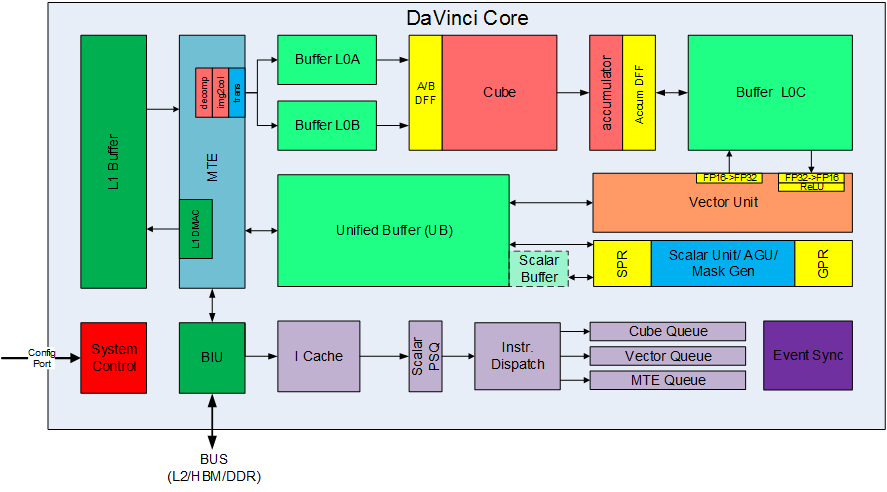
\includegraphics[scale=0.5]{DaVinci.png}
    \caption{Архитектура DaVinci}
\end{figure}

В ядре есть три вычислительных юнита: матричный, векторный и скалярный,
которые используются для соответствующих вычилений.  Исполнение на юнитах
происходит параллельно, для каждого юнита существует
отдельная, независимая очередь задач. Ещё три очереди предназначены для
копирования из разных буфферов друг в друга (о них речь пойдёт ниже).
Для синхронизации очередей используются команды \texttt{set\_flag} и \texttt{wait\_flag},
которые по своей сути представляют систему событий. Первая команда сигнализирует,
что событие произошло, а вторая запускает ожидание события. Правильное
использование механизмов синхронизации позволяет значительно увеличить
загрузку всех юнитов и, следовательно, снизить общее время исполнения.
В данной работе не будут рассматривать проблемы с расстановкой операций
синхронизации и будет считаться, что они всегда расставлены наиболее
оптимальным образом.

Матричный юнит на вход принимает матрицы с типом элементов \texttt{float 16}
или \texttt{int 8}, на выходе же элементы имеют тип \texttt{float 16},
\texttt{float 32} или \texttt{int 32}. Умножение работает в двух режимах:

\begin{enumerate}
    \item Обычное умножение: $C = A \times B$
    \item Режим накопления: $C = A \times B + C$, т.~е. результат текущего
          умножения прибавляется к предыдущему.
\end{enumerate}

Каждая из входных матриц должна быть разбита на блоки $16 \times 16$
(в случае \texttt{float 16}) или $16 \times 32$ (в случае \texttt{int 8}).
Расположение элементов внутри блоков и блоков относительно друг друга также
различно. Существуют две стратегии размещения: про строкам (формат \texttt{Z})
и по столбцам (формат \texttt{N}). Примем обозначение: размещение внутри блока
обозначается строчной буквой, а между блоками --- заглавной. При умножении
матрица $A$ должна быть заранее быть записана в формате \texttt{Zz},
матрица $B$ --- в формате \texttt{Zn}, а выходная матрица $C$ будет \texttt{Nz}.

Во-первых, память ядра неоднородна. В ядре существует 5 буферов:
L1, L0A, L0B, L0C, UB. Также существует внешняя память (GM), через которую
происходит общение с хостом. Опишем общую схему потока данных между этими кэшами.
Данные из внешней памяти загружаются в L1 и UB. Данные в UB предназначены для
обработки векторным и скалярным юнитами. Данные из L1 загружаются в L0A и L0B,
которые соответствуют матрицам A и B матричного умножения. Результат после
перемножения (которое, как было упомянуто раньше, выполняется матричным юнитом),
попадает в буфер L0C, из которого происходит данные отправляются в UB. Выгрузка
результата вычислений во внешнюю память возможна только из UB. Отметим, что
описанные выше буферы имеют небольшой размер, что является одной из основных
проблематик нашей работы. Более подробно этот вопрос будет рассмотрен в главе,
посвященной ловерингу.

Отдельно стоит рассмотреть устройство матричного юнита, который представляет
из себя систолический массив. Систолический массив --- однородная сеть тесно
связанных блоков обработки данных. Его схему для архитектуры DaVinci можно
увидеть на картинке ниже. 

\begin{figure}[h!]
    \centering
    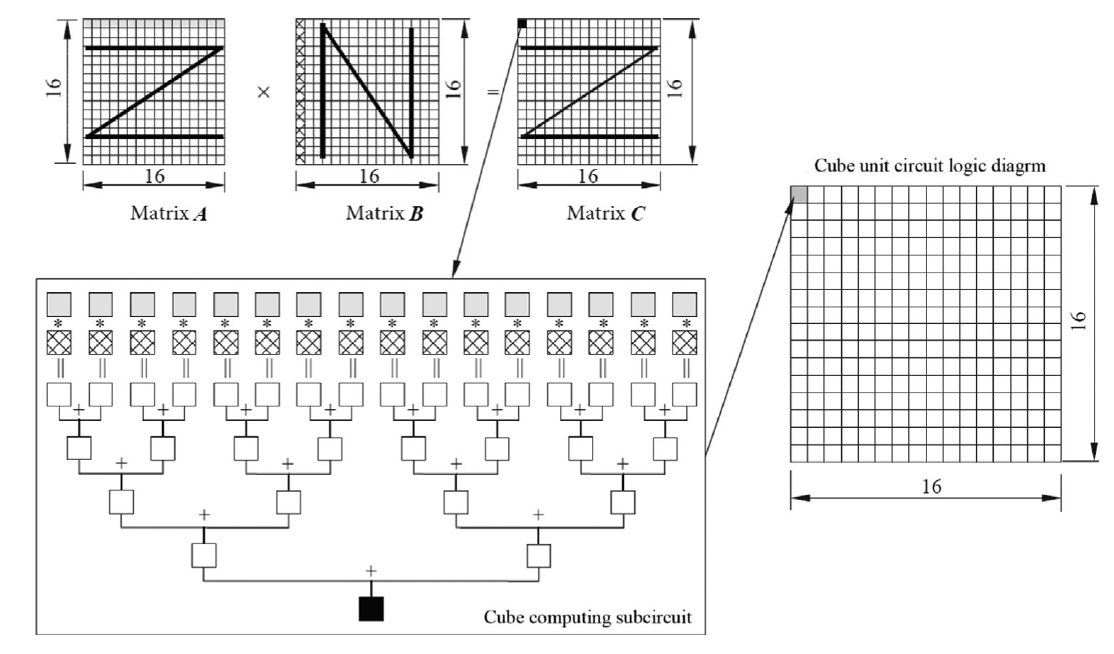
\includegraphics[scale=0.5]{Systolic.png}
    \caption{Схема вычисления в матричном юните}
\end{figure}

Принцип умножения довольно прост: за первый такт (FIXME: лучше не использовать
слово такт в данном контексте) происходят все умножения,
после чего за оставшиеся четыре такта произведения суммируются. Таким
образом, за пять тактов можно перемножить две матрицы \texttt{16x16}.
Матричный юнит, итерируясь по матрицам и перемножая их поблочно, быстро
получает результат перемножения.

Процессоры, основанные на архитектуре DaVinci и их основные характеристики
представлены в таблице ниже:

FIXME

\newpage
